
% Default to the notebook output style

    


% Inherit from the specified cell style.




    
\documentclass[11pt]{article}

    
    
    \usepackage[T1]{fontenc}
    % Nicer default font (+ math font) than Computer Modern for most use cases
    \usepackage{mathpazo}
    \usepackage{float}

    % Basic figure setup, for now with no caption control since it's done
    % automatically by Pandoc (which extracts ![](path) syntax from Markdown).
    \usepackage{graphicx}
    % We will generate all images so they have a width \maxwidth. This means
    % that they will get their normal width if they fit onto the page, but
    % are scaled down if they would overflow the margins.
    \makeatletter
    \def\maxwidth{\ifdim\Gin@nat@width>\linewidth\linewidth
    \else\Gin@nat@width\fi}
    \makeatother
    \let\Oldincludegraphics\includegraphics
    % Set max figure width to be 80% of text width, for now hardcoded.
    \renewcommand{\includegraphics}[1]{\Oldincludegraphics[width=.8\maxwidth]{#1}}
    % Ensure that by default, figures have no caption (until we provide a
    % proper Figure object with a Caption API and a way to capture that
    % in the conversion process - todo).
    \usepackage{caption}
    \DeclareCaptionLabelFormat{nolabel}{}
    \captionsetup{labelformat=nolabel}

    \usepackage{adjustbox} % Used to constrain images to a maximum size 
    \usepackage{xcolor} % Allow colors to be defined
    \usepackage{enumerate} % Needed for markdown enumerations to work
    \usepackage{geometry} % Used to adjust the document margins
    \usepackage{amsmath} % Equations
    \usepackage{amssymb} % Equations
    \usepackage{textcomp} % defines textquotesingle
    % Hack from http://tex.stackexchange.com/a/47451/13684:
    \AtBeginDocument{%
        \def\PYZsq{\textquotesingle}% Upright quotes in Pygmentized code
    }
    \usepackage{upquote} % Upright quotes for verbatim code
    \usepackage{eurosym} % defines \euro
    \usepackage[mathletters]{ucs} % Extended unicode (utf-8) support
    \usepackage[utf8x]{inputenc} % Allow utf-8 characters in the tex document
    \usepackage{fancyvrb} % verbatim replacement that allows latex
    \usepackage{grffile} % extends the file name processing of package graphics 
                         % to support a larger range 
    % The hyperref package gives us a pdf with properly built
    % internal navigation ('pdf bookmarks' for the table of contents,
    % internal cross-reference links, web links for URLs, etc.)
    \usepackage{hyperref}
    \usepackage{longtable} % longtable support required by pandoc >1.10
    \usepackage{booktabs}  % table support for pandoc > 1.12.2
    \usepackage[inline]{enumitem} % IRkernel/repr support (it uses the enumerate* environment)
    \usepackage[normalem]{ulem} % ulem is needed to support strikethroughs (\sout)
                                % normalem makes italics be italics, not underlines
    

    
    
    % Colors for the hyperref package
    \definecolor{urlcolor}{rgb}{0,.145,.698}
    \definecolor{linkcolor}{rgb}{.71,0.21,0.01}
    \definecolor{citecolor}{rgb}{.12,.54,.11}

    % ANSI colors
    \definecolor{ansi-black}{HTML}{3E424D}
    \definecolor{ansi-black-intense}{HTML}{282C36}
    \definecolor{ansi-red}{HTML}{E75C58}
    \definecolor{ansi-red-intense}{HTML}{B22B31}
    \definecolor{ansi-green}{HTML}{00A250}
    \definecolor{ansi-green-intense}{HTML}{007427}
    \definecolor{ansi-yellow}{HTML}{DDB62B}
    \definecolor{ansi-yellow-intense}{HTML}{B27D12}
    \definecolor{ansi-blue}{HTML}{208FFB}
    \definecolor{ansi-blue-intense}{HTML}{0065CA}
    \definecolor{ansi-magenta}{HTML}{D160C4}
    \definecolor{ansi-magenta-intense}{HTML}{A03196}
    \definecolor{ansi-cyan}{HTML}{60C6C8}
    \definecolor{ansi-cyan-intense}{HTML}{258F8F}
    \definecolor{ansi-white}{HTML}{C5C1B4}
    \definecolor{ansi-white-intense}{HTML}{A1A6B2}

    % commands and environments needed by pandoc snippets
    % extracted from the output of `pandoc -s`
    \providecommand{\tightlist}{%
      \setlength{\itemsep}{0pt}\setlength{\parskip}{0pt}}
    \DefineVerbatimEnvironment{Highlighting}{Verbatim}{commandchars=\\\{\}}
    % Add ',fontsize=\small' for more characters per line
    \newenvironment{Shaded}{}{}
    \newcommand{\KeywordTok}[1]{\textcolor[rgb]{0.00,0.44,0.13}{\textbf{{#1}}}}
    \newcommand{\DataTypeTok}[1]{\textcolor[rgb]{0.56,0.13,0.00}{{#1}}}
    \newcommand{\DecValTok}[1]{\textcolor[rgb]{0.25,0.63,0.44}{{#1}}}
    \newcommand{\BaseNTok}[1]{\textcolor[rgb]{0.25,0.63,0.44}{{#1}}}
    \newcommand{\FloatTok}[1]{\textcolor[rgb]{0.25,0.63,0.44}{{#1}}}
    \newcommand{\CharTok}[1]{\textcolor[rgb]{0.25,0.44,0.63}{{#1}}}
    \newcommand{\StringTok}[1]{\textcolor[rgb]{0.25,0.44,0.63}{{#1}}}
    \newcommand{\CommentTok}[1]{\textcolor[rgb]{0.38,0.63,0.69}{\textit{{#1}}}}
    \newcommand{\OtherTok}[1]{\textcolor[rgb]{0.00,0.44,0.13}{{#1}}}
    \newcommand{\AlertTok}[1]{\textcolor[rgb]{1.00,0.00,0.00}{\textbf{{#1}}}}
    \newcommand{\FunctionTok}[1]{\textcolor[rgb]{0.02,0.16,0.49}{{#1}}}
    \newcommand{\RegionMarkerTok}[1]{{#1}}
    \newcommand{\ErrorTok}[1]{\textcolor[rgb]{1.00,0.00,0.00}{\textbf{{#1}}}}
    \newcommand{\NormalTok}[1]{{#1}}
    
    % Additional commands for more recent versions of Pandoc
    \newcommand{\ConstantTok}[1]{\textcolor[rgb]{0.53,0.00,0.00}{{#1}}}
    \newcommand{\SpecialCharTok}[1]{\textcolor[rgb]{0.25,0.44,0.63}{{#1}}}
    \newcommand{\VerbatimStringTok}[1]{\textcolor[rgb]{0.25,0.44,0.63}{{#1}}}
    \newcommand{\SpecialStringTok}[1]{\textcolor[rgb]{0.73,0.40,0.53}{{#1}}}
    \newcommand{\ImportTok}[1]{{#1}}
    \newcommand{\DocumentationTok}[1]{\textcolor[rgb]{0.73,0.13,0.13}{\textit{{#1}}}}
    \newcommand{\AnnotationTok}[1]{\textcolor[rgb]{0.38,0.63,0.69}{\textbf{\textit{{#1}}}}}
    \newcommand{\CommentVarTok}[1]{\textcolor[rgb]{0.38,0.63,0.69}{\textbf{\textit{{#1}}}}}
    \newcommand{\VariableTok}[1]{\textcolor[rgb]{0.10,0.09,0.49}{{#1}}}
    \newcommand{\ControlFlowTok}[1]{\textcolor[rgb]{0.00,0.44,0.13}{\textbf{{#1}}}}
    \newcommand{\OperatorTok}[1]{\textcolor[rgb]{0.40,0.40,0.40}{{#1}}}
    \newcommand{\BuiltInTok}[1]{{#1}}
    \newcommand{\ExtensionTok}[1]{{#1}}
    \newcommand{\PreprocessorTok}[1]{\textcolor[rgb]{0.74,0.48,0.00}{{#1}}}
    \newcommand{\AttributeTok}[1]{\textcolor[rgb]{0.49,0.56,0.16}{{#1}}}
    \newcommand{\InformationTok}[1]{\textcolor[rgb]{0.38,0.63,0.69}{\textbf{\textit{{#1}}}}}
    \newcommand{\WarningTok}[1]{\textcolor[rgb]{0.38,0.63,0.69}{\textbf{\textit{{#1}}}}}
    
    
    % Define a nice break command that doesn't care if a line doesn't already
    % exist.
    \def\br{\hspace*{\fill} \\* }
    % Math Jax compatability definitions
    \def\gt{>}
    \def\lt{<}
    % Document parameters
    \title{Problemset 2: K Nearest Neighbor and Linear
Regression}
    \author{Jiarong Ye}
    
    

    % Pygments definitions
    
\makeatletter
\def\PY@reset{\let\PY@it=\relax \let\PY@bf=\relax%
    \let\PY@ul=\relax \let\PY@tc=\relax%
    \let\PY@bc=\relax \let\PY@ff=\relax}
\def\PY@tok#1{\csname PY@tok@#1\endcsname}
\def\PY@toks#1+{\ifx\relax#1\empty\else%
    \PY@tok{#1}\expandafter\PY@toks\fi}
\def\PY@do#1{\PY@bc{\PY@tc{\PY@ul{%
    \PY@it{\PY@bf{\PY@ff{#1}}}}}}}
\def\PY#1#2{\PY@reset\PY@toks#1+\relax+\PY@do{#2}}

\expandafter\def\csname PY@tok@nv\endcsname{\def\PY@tc##1{\textcolor[rgb]{0.10,0.09,0.49}{##1}}}
\expandafter\def\csname PY@tok@kr\endcsname{\let\PY@bf=\textbf\def\PY@tc##1{\textcolor[rgb]{0.00,0.50,0.00}{##1}}}
\expandafter\def\csname PY@tok@kd\endcsname{\let\PY@bf=\textbf\def\PY@tc##1{\textcolor[rgb]{0.00,0.50,0.00}{##1}}}
\expandafter\def\csname PY@tok@kp\endcsname{\def\PY@tc##1{\textcolor[rgb]{0.00,0.50,0.00}{##1}}}
\expandafter\def\csname PY@tok@nt\endcsname{\let\PY@bf=\textbf\def\PY@tc##1{\textcolor[rgb]{0.00,0.50,0.00}{##1}}}
\expandafter\def\csname PY@tok@gh\endcsname{\let\PY@bf=\textbf\def\PY@tc##1{\textcolor[rgb]{0.00,0.00,0.50}{##1}}}
\expandafter\def\csname PY@tok@kt\endcsname{\def\PY@tc##1{\textcolor[rgb]{0.69,0.00,0.25}{##1}}}
\expandafter\def\csname PY@tok@c\endcsname{\let\PY@it=\textit\def\PY@tc##1{\textcolor[rgb]{0.25,0.50,0.50}{##1}}}
\expandafter\def\csname PY@tok@cpf\endcsname{\let\PY@it=\textit\def\PY@tc##1{\textcolor[rgb]{0.25,0.50,0.50}{##1}}}
\expandafter\def\csname PY@tok@nd\endcsname{\def\PY@tc##1{\textcolor[rgb]{0.67,0.13,1.00}{##1}}}
\expandafter\def\csname PY@tok@se\endcsname{\let\PY@bf=\textbf\def\PY@tc##1{\textcolor[rgb]{0.73,0.40,0.13}{##1}}}
\expandafter\def\csname PY@tok@vi\endcsname{\def\PY@tc##1{\textcolor[rgb]{0.10,0.09,0.49}{##1}}}
\expandafter\def\csname PY@tok@sh\endcsname{\def\PY@tc##1{\textcolor[rgb]{0.73,0.13,0.13}{##1}}}
\expandafter\def\csname PY@tok@ch\endcsname{\let\PY@it=\textit\def\PY@tc##1{\textcolor[rgb]{0.25,0.50,0.50}{##1}}}
\expandafter\def\csname PY@tok@bp\endcsname{\def\PY@tc##1{\textcolor[rgb]{0.00,0.50,0.00}{##1}}}
\expandafter\def\csname PY@tok@o\endcsname{\def\PY@tc##1{\textcolor[rgb]{0.40,0.40,0.40}{##1}}}
\expandafter\def\csname PY@tok@gs\endcsname{\let\PY@bf=\textbf}
\expandafter\def\csname PY@tok@gt\endcsname{\def\PY@tc##1{\textcolor[rgb]{0.00,0.27,0.87}{##1}}}
\expandafter\def\csname PY@tok@gp\endcsname{\let\PY@bf=\textbf\def\PY@tc##1{\textcolor[rgb]{0.00,0.00,0.50}{##1}}}
\expandafter\def\csname PY@tok@il\endcsname{\def\PY@tc##1{\textcolor[rgb]{0.40,0.40,0.40}{##1}}}
\expandafter\def\csname PY@tok@err\endcsname{\def\PY@bc##1{\setlength{\fboxsep}{0pt}\fcolorbox[rgb]{1.00,0.00,0.00}{1,1,1}{\strut ##1}}}
\expandafter\def\csname PY@tok@kc\endcsname{\let\PY@bf=\textbf\def\PY@tc##1{\textcolor[rgb]{0.00,0.50,0.00}{##1}}}
\expandafter\def\csname PY@tok@cs\endcsname{\let\PY@it=\textit\def\PY@tc##1{\textcolor[rgb]{0.25,0.50,0.50}{##1}}}
\expandafter\def\csname PY@tok@ne\endcsname{\let\PY@bf=\textbf\def\PY@tc##1{\textcolor[rgb]{0.82,0.25,0.23}{##1}}}
\expandafter\def\csname PY@tok@nl\endcsname{\def\PY@tc##1{\textcolor[rgb]{0.63,0.63,0.00}{##1}}}
\expandafter\def\csname PY@tok@dl\endcsname{\def\PY@tc##1{\textcolor[rgb]{0.73,0.13,0.13}{##1}}}
\expandafter\def\csname PY@tok@ow\endcsname{\let\PY@bf=\textbf\def\PY@tc##1{\textcolor[rgb]{0.67,0.13,1.00}{##1}}}
\expandafter\def\csname PY@tok@cp\endcsname{\def\PY@tc##1{\textcolor[rgb]{0.74,0.48,0.00}{##1}}}
\expandafter\def\csname PY@tok@cm\endcsname{\let\PY@it=\textit\def\PY@tc##1{\textcolor[rgb]{0.25,0.50,0.50}{##1}}}
\expandafter\def\csname PY@tok@go\endcsname{\def\PY@tc##1{\textcolor[rgb]{0.53,0.53,0.53}{##1}}}
\expandafter\def\csname PY@tok@fm\endcsname{\def\PY@tc##1{\textcolor[rgb]{0.00,0.00,1.00}{##1}}}
\expandafter\def\csname PY@tok@mf\endcsname{\def\PY@tc##1{\textcolor[rgb]{0.40,0.40,0.40}{##1}}}
\expandafter\def\csname PY@tok@nn\endcsname{\let\PY@bf=\textbf\def\PY@tc##1{\textcolor[rgb]{0.00,0.00,1.00}{##1}}}
\expandafter\def\csname PY@tok@sc\endcsname{\def\PY@tc##1{\textcolor[rgb]{0.73,0.13,0.13}{##1}}}
\expandafter\def\csname PY@tok@mb\endcsname{\def\PY@tc##1{\textcolor[rgb]{0.40,0.40,0.40}{##1}}}
\expandafter\def\csname PY@tok@mh\endcsname{\def\PY@tc##1{\textcolor[rgb]{0.40,0.40,0.40}{##1}}}
\expandafter\def\csname PY@tok@s2\endcsname{\def\PY@tc##1{\textcolor[rgb]{0.73,0.13,0.13}{##1}}}
\expandafter\def\csname PY@tok@mi\endcsname{\def\PY@tc##1{\textcolor[rgb]{0.40,0.40,0.40}{##1}}}
\expandafter\def\csname PY@tok@si\endcsname{\let\PY@bf=\textbf\def\PY@tc##1{\textcolor[rgb]{0.73,0.40,0.53}{##1}}}
\expandafter\def\csname PY@tok@m\endcsname{\def\PY@tc##1{\textcolor[rgb]{0.40,0.40,0.40}{##1}}}
\expandafter\def\csname PY@tok@s1\endcsname{\def\PY@tc##1{\textcolor[rgb]{0.73,0.13,0.13}{##1}}}
\expandafter\def\csname PY@tok@sa\endcsname{\def\PY@tc##1{\textcolor[rgb]{0.73,0.13,0.13}{##1}}}
\expandafter\def\csname PY@tok@ss\endcsname{\def\PY@tc##1{\textcolor[rgb]{0.10,0.09,0.49}{##1}}}
\expandafter\def\csname PY@tok@no\endcsname{\def\PY@tc##1{\textcolor[rgb]{0.53,0.00,0.00}{##1}}}
\expandafter\def\csname PY@tok@ge\endcsname{\let\PY@it=\textit}
\expandafter\def\csname PY@tok@k\endcsname{\let\PY@bf=\textbf\def\PY@tc##1{\textcolor[rgb]{0.00,0.50,0.00}{##1}}}
\expandafter\def\csname PY@tok@sd\endcsname{\let\PY@it=\textit\def\PY@tc##1{\textcolor[rgb]{0.73,0.13,0.13}{##1}}}
\expandafter\def\csname PY@tok@s\endcsname{\def\PY@tc##1{\textcolor[rgb]{0.73,0.13,0.13}{##1}}}
\expandafter\def\csname PY@tok@vm\endcsname{\def\PY@tc##1{\textcolor[rgb]{0.10,0.09,0.49}{##1}}}
\expandafter\def\csname PY@tok@gu\endcsname{\let\PY@bf=\textbf\def\PY@tc##1{\textcolor[rgb]{0.50,0.00,0.50}{##1}}}
\expandafter\def\csname PY@tok@gd\endcsname{\def\PY@tc##1{\textcolor[rgb]{0.63,0.00,0.00}{##1}}}
\expandafter\def\csname PY@tok@w\endcsname{\def\PY@tc##1{\textcolor[rgb]{0.73,0.73,0.73}{##1}}}
\expandafter\def\csname PY@tok@nb\endcsname{\def\PY@tc##1{\textcolor[rgb]{0.00,0.50,0.00}{##1}}}
\expandafter\def\csname PY@tok@sr\endcsname{\def\PY@tc##1{\textcolor[rgb]{0.73,0.40,0.53}{##1}}}
\expandafter\def\csname PY@tok@gi\endcsname{\def\PY@tc##1{\textcolor[rgb]{0.00,0.63,0.00}{##1}}}
\expandafter\def\csname PY@tok@ni\endcsname{\let\PY@bf=\textbf\def\PY@tc##1{\textcolor[rgb]{0.60,0.60,0.60}{##1}}}
\expandafter\def\csname PY@tok@sb\endcsname{\def\PY@tc##1{\textcolor[rgb]{0.73,0.13,0.13}{##1}}}
\expandafter\def\csname PY@tok@gr\endcsname{\def\PY@tc##1{\textcolor[rgb]{1.00,0.00,0.00}{##1}}}
\expandafter\def\csname PY@tok@mo\endcsname{\def\PY@tc##1{\textcolor[rgb]{0.40,0.40,0.40}{##1}}}
\expandafter\def\csname PY@tok@na\endcsname{\def\PY@tc##1{\textcolor[rgb]{0.49,0.56,0.16}{##1}}}
\expandafter\def\csname PY@tok@c1\endcsname{\let\PY@it=\textit\def\PY@tc##1{\textcolor[rgb]{0.25,0.50,0.50}{##1}}}
\expandafter\def\csname PY@tok@nc\endcsname{\let\PY@bf=\textbf\def\PY@tc##1{\textcolor[rgb]{0.00,0.00,1.00}{##1}}}
\expandafter\def\csname PY@tok@nf\endcsname{\def\PY@tc##1{\textcolor[rgb]{0.00,0.00,1.00}{##1}}}
\expandafter\def\csname PY@tok@vg\endcsname{\def\PY@tc##1{\textcolor[rgb]{0.10,0.09,0.49}{##1}}}
\expandafter\def\csname PY@tok@sx\endcsname{\def\PY@tc##1{\textcolor[rgb]{0.00,0.50,0.00}{##1}}}
\expandafter\def\csname PY@tok@vc\endcsname{\def\PY@tc##1{\textcolor[rgb]{0.10,0.09,0.49}{##1}}}
\expandafter\def\csname PY@tok@kn\endcsname{\let\PY@bf=\textbf\def\PY@tc##1{\textcolor[rgb]{0.00,0.50,0.00}{##1}}}

\def\PYZbs{\char`\\}
\def\PYZus{\char`\_}
\def\PYZob{\char`\{}
\def\PYZcb{\char`\}}
\def\PYZca{\char`\^}
\def\PYZam{\char`\&}
\def\PYZlt{\char`\<}
\def\PYZgt{\char`\>}
\def\PYZsh{\char`\#}
\def\PYZpc{\char`\%}
\def\PYZdl{\char`\$}
\def\PYZhy{\char`\-}
\def\PYZsq{\char`\'}
\def\PYZdq{\char`\"}
\def\PYZti{\char`\~}
% for compatibility with earlier versions
\def\PYZat{@}
\def\PYZlb{[}
\def\PYZrb{]}
\makeatother


    % Exact colors from NB
    \definecolor{incolor}{rgb}{0.0, 0.0, 0.5}
    \definecolor{outcolor}{rgb}{0.545, 0.0, 0.0}



    
    % Prevent overflowing lines due to hard-to-break entities
    \sloppy 
    % Setup hyperref package
    \hypersetup{
      breaklinks=true,  % so long urls are correctly broken across lines
      colorlinks=true,
      urlcolor=urlcolor,
      linkcolor=linkcolor,
      citecolor=citecolor,
      }
    % Slightly bigger margins than the latex defaults
    
    \geometry{verbose,tmargin=1in,bmargin=1in,lmargin=1in,rmargin=1in}
    
    

    \begin{document}
    
    
    \maketitle
    
    

    \subsubsection*{Q1}\label{q1}

    1.(25 pts.) Suppose 7 nearest neighbor search for a query sample returns
\{7, 6, 8, 4, 7, 11, 9\} as the values of the function at the 7 nearest
data samples in the training set.

(a) Assuming prediction using 7 nearest neighbor interpolation, what is
    the predicted value of the function for the query sample?

(b) Assuming prediction using 7 nearest neighbor regression, what is the
    predicted value of the function for the query sample?


    \begin{itemize}
\item
  \begin{enumerate}
  \def\labelenumi{(\alph{enumi})}
  \tightlist
  \item
    Since the nearest neighbor interpolation selects the value of the
    nearest point and does not consider other values of neighboring points
    at all, thus \(\arg \min distance(x', x_i)\) is achieved at \(i\)
    when \(f(x_i)=7\), thus the predicted value of the function for the
    sample \(x'\) should be \(7\)
  \end{enumerate}
\end{itemize}

    \begin{itemize}
\item
  \begin{enumerate}
  \def\labelenumi{(\alph{enumi})}
  \setcounter{enumi}{1}
  \tightlist
  \item
    the result depends on the loss function applied, for instance:
  \end{enumerate}

  \begin{itemize}
  \tightlist
  \item[*]
    L1 loss \[\min \frac{1}{n} \sum^n_{i=1} \mid f(x') - f(x_i) \mid\]
  \end{itemize}

  in this case

\begin{equation*}
	\begin{aligned}
		\arg \min \left \{\mid f(x') - 7 \mid + \mid f(x') - 6 \mid +\mid f(x') - 8 \mid+\mid (x') - 4 \mid \\
		+\mid f(x') - 7 \mid +\mid f(x') - 11 \mid+\mid f(x') - 9 \mid  \} 
	\end{aligned}
\end{equation*}


  is achieved when  \(f(x')\) is the median of the array, thus the predicted value of the function for the sample \(x'\) should
  be \(7\)

  \begin{itemize}
  \tightlist
  \item[*]
    L2 loss
  \end{itemize}

  \[\min L , \: where \: L = \frac{1}{n} \sum^n_{i=1} \left ( f(x') - f(x_i) \right )^2\]

  in this case

\begin{equation*}
	\begin{aligned}
	\arg \min  \{\left ( f(x') - 7\right )^2+ \left ( f(x') - 6 \right )^2+ \left ( f(x') - 8 \right )^2+ \left ( f(x') - 4 \right )^2+\\ \left ( f(x') - 7 \right )^2+ \left ( f(x') - 11 \right )^2+ \left ( f(x') -9 \right )^2 \}
	\end{aligned}
\end{equation*}

  is achieved when

 \begin{equation*}\label{eq:}
 \begin{aligned}
 \frac{\partial L}{\partial f(x')} = 2 [\left ( f(x') - 7 \right ) + \left ( f(x') - 6 \right )+ 
  \left ( f(x') - 8 \right )+ 
   \left ( f(x') - 4 \right )+ \\
    \left ( f(x') - 7\right )+ \left ( f(x') -11 \right )+ \left ( f(x') - 9 ]\right ]
  \end{aligned}
 \end{equation*}
 
 \begin{equation*}
 	=14 f(x') -2 \cdot 52 = 0
 \end{equation*}

  \[f(x') = 7.429\]

  (\textbf{also the mean of the array})

  thus the predicted value of the function for the sample \(x'\) should
  be \(7.429\)
\end{itemize}

    \subsubsection*{Q2}\label{q2}

    2.(25 pts.) Alex is building a K nearest neighbor classifier for
predicting the language to which a word belongs. The words use the Latin
alphabet (which is used by English, Spanish, German and several other
European languages). For better or for worse, Alex chooses to represent
the words using three features: length of the word, number of vowels in
the word, and whether or not the word ends in the letter 'n'' (0 for No,
1 for Yes). Suppose she has training data for two languages: regeln:
German; pido: spanish.

(a) What is the dimensionality of the feature space?
 
(b) How are the two training data samples encoded in terms of the 3
    features listed?

(c) Using 1-nearest neighbor classifier using the Manhattan distance
    metric, what is the prediction for the word ''neben''?


    \begin{itemize}
\item
  \begin{enumerate}
  \def\labelenumi{(\alph{enumi})}
  \tightlist
  \item
    The dimensionality of the feature space is 3 because there are three
    engineered features in feature set:
  \end{enumerate}

  \begin{itemize}
  \tightlist
  \item[*]
    length of the word
  \item[*]
    number of vowels in the word
  \item[*]
    whether or not the word ends in the letter 'n'
  \end{itemize}
\item
  \begin{enumerate}
  \def\labelenumi{(\alph{enumi})}
  \setcounter{enumi}{1}
  \item
  \end{enumerate}
\end{itemize}

\begin{center}
	\begin{tabular}{||c |c |c | c||} 
		\hline
		sample & length of word & number of vowels in the word & whether or not the word ends in the letter 'n'\\ [0.5ex] 
		\hline\hline
		regeln & 6 & 2 & 1 \\ 
		\hline
		pido & 4 & 2 & 0 \\
		\hline
	\end{tabular}
\end{center}

\begin{itemize}
\item
  \begin{enumerate}
  \def\labelenumi{(\alph{enumi})}
  \setcounter{enumi}{2}
  \item
  \end{enumerate}
\end{itemize}

the feature encoding for 'neben' is:

\begin{center}
	\begin{tabular}{||c |c |c | c||} 
		\hline
		sample & length of word & number of vowels in the word & whether or not the word ends in the letter 'n'\\ [0.5ex] 
		\hline\hline
		neben & 5 & 2 & 1 \\ 
		\hline
	\end{tabular}
\end{center}




Using the Manhattan distance metric:

\[distance = \left|x_{1}-x_{2}\right|+\left|y_{1}-y_{2}\right|+\left|z_{1}-z_{2}\right|\]

Therefore:

\begin{itemize}
\tightlist
\item
  'neben' to 'regeln':
\end{itemize}

\[distance_1 = \left|5-6\right|+\left|2-2\right|+\left|1-1\right| = 1\]

\begin{itemize}
\tightlist
\item
  'neben' to 'pido':
\end{itemize}

\[distance_2 = \left|5-4\right|+\left|2-2\right|+\left|1-0\right| = 2\]

So:

\[\min (distance_1, distance_2) = distance_1 = 1\]

Thus 'neben' is more likely to be German.

    \subsubsection*{Q3}\label{q3}

    3.(25 pts.) Assume that you have a trained K nearest neighbor
classifier.

(a) What is the runtime complexity of this classifying p data samples
    given a K nearest neighbor classifier trained on m training samples,
    each represented using d features?.

(b) Can you do better, using a carefully designed data structure with a
    K nearest neighbor search algorithm that is designed to take
    advantage of the data structure? Explain.\\\\

\noindent (a)
Explain by steps:

\begin{itemize}
\item
  for each of the p data samples:

  \begin{itemize}
  \item[*]
    step 1: distance with each of the training data points need to be
    calculated for later comparison, each calculation takes \(O(d)\),
    thus for all m training data points, the runtime complexity is
    \(O(dm)\)
  \item[*]
    step 2: then for the top K required nearest neighbors 1 to k, each loop through all \(m\) distance factor calculated, selecting the index with the smallest distance, the runtime complexity is \(O(km)\)
  \end{itemize}
\end{itemize}

\noindent \textbf{Summary: }

for each of the p data samples, a classification task takes runtime
complexity of \(O(dm) + O(km)\);

for total p samples, the runtime complexity is \(O((d+k)mp)\)\\\

\noindent (b)
    As we can see, the part where we probably could optimize the runtime
    complexity would be \textbf{step 2} where in part (a), we traverse
    the entire  \(m\) calculated distance factor to search the shortest distance, costing \(O(km)\) complexity\\

\noindent we could use a more carefully designed data structure, like the
\textbf{KD-Tree} for this part in the KNN search algorithm by organize
the m training data points into different segmentations.\\

\noindent Basically how KD-Tree works:

\begin{itemize}
\item
  If there is just one point, form a leaf with that point.
\item
  Otherwise, divide the points in half by a line perpendicular to one of
  the axes.
\item
  Recursively construct k-d trees for the two sets of points.
\end{itemize}



 \noindent Runtime complexity of searching for top K nearest neighbors:\\

Since \(depth \: of \: KDTree = \log m\) \\

\noindent for each of the p data samples:
\begin{itemize}
\tightlist
\item 
	each distance calculation with m training data points takes \(O(d)\),
	thus for all m training data points, the runtime complexity is
	\(O(dm)\)
\item
   for the top K required nearest neighbors 1 to k, each takes \(O( \log m)\) to traverse the tree and extract the shortest distance, then the runtime complexity is \(O(k \log m)\)
\end{itemize}

\noindent \textbf{Summary: }

\begin{itemize}
\tightlist
\item
  If construct a KD-Tree to organize the training data first then do the
  knn search

  \begin{itemize}
  \tightlist
  \item[*]
    the runtime complexity for knn searching is \(O(k \log m)\)
    \item[*]
    the whole runtime complexity of the adjusted KNN algorithm for p samples is 
    \(O((dm+k \log m)p)\)
  \end{itemize}
\end{itemize}

    \subsubsection*{Q4}\label{q4}

    4.(25pts.)Consider approximation of \(f(X)\) where
\(X \in \mathbb{R}^d\) given a training set
\(\{(X_1, y_1), ..., (X_n, y_n)\}\) using linear regression. That is,
the goal is to find a linear approximation \(y(X) = W \cdot X + w_0\)
where \(W\) and \(w_0\) are learnable parameters. Suppose we further
know that the function is sparse, i.e., only a few of the d features
define the behavior of f. How would you modify the objective function to
be minimized to ensure that the resulting linear is sparse? (Hint: Add a
term to the mean squared error that when minimized attempts to drive the
weights to 0).\\\\

\noindent    Since the function is sparse, with a few among all \(d\) features that
actually non-zero, thus to make sure the resulting linear is sparse as
well, we could modify the loss function by adding a regularization term,
a smoothing technique to prevent overfitting by bounding the weights.
And in this case, to drive the weights to 0, it would be better if the
added regularization term is \textbf{L1 regularization}.

\[L = \frac{1}{n} \sum^n_{i=1} (y_i - \hat {y_i})^2 = \frac{1}{n} \sum^n_{i=1} (y_i - \sum_{j=1}w_j \cdot x_{ij} -w_0)^2\]

\noindent Objective function:

\[\arg \min _w \left \{ L + \lambda ||w||_1 \right \}\]

\noindent \textbf{Explain}:

 L1 regularization is better for sparse fucntion, because it is
more likely to create 0-weights:


\begin{itemize}
\tightlist
\item
  mathematical proof:
\end{itemize}

for a model consisting of the weights \((w_1,w_2,...,w_m)\)

\begin{enumerate}
\def\labelenumi{\arabic{enumi}.}
\item
  With L1 regularization, the loss function
  \(L_1(w) = f(w) + \lambda||w||_1\)
\item
  With L2 regularization, the loss function
  \(L_2(w) = f(w) +\lambda ||w||^2_2\)
\end{enumerate}



\[\frac{\partial L_1}{\partial w} = f(w)' + \lambda \cdot \frac{w}{|w|}, \: where \: \frac{w}{|w|} = \pm 1\]

Optimization theory says that the optimum of a function is either the point with 0-derivative or one of the irregularities (corners, kinks, etc.). So, it's possible that the optimal point of L is 0 even if 0 isn't the 0-derivative of \(f(w)\). In fact, it would be 0 if \(\lambda\) is large enough (stronger regularization effect). 

\[\frac{\partial L_2}{\partial w} = f(w)' + 2 \lambda w\]

\[w = w - \eta \cdot \frac{\partial L}{\partial w}, \: where \: \frac{\partial L}{\partial w}  is \: dependent \: to \: w\]

So in L2 regularization, gradient \(\frac{L_2}{w}\) is linearly
decreasing towards 0 as the weight goes towards 0. Therefore, it will
take smaller and smaller steps as a weight approaches 0.
 The 0-derivative point of \(L_2\) can get very small when  \(\lambda\) increases, but still won't be 0 unless  f'(0)=0

\begin{itemize}
\tightlist
\item
  intuition:
\end{itemize}

\begin{figure}[H]
\centering
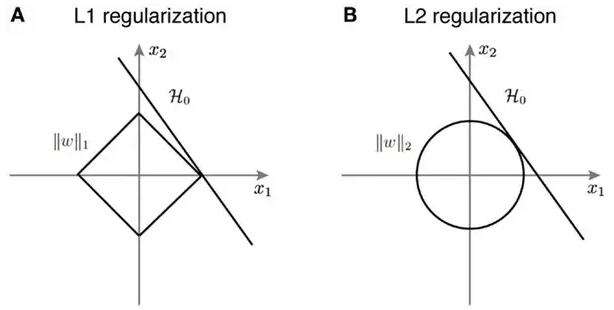
\includegraphics{l1l2.png}
\caption{}
\end{figure}

As the objective is to minimize the error function,
we then focus on the intersection with the L1, L2
regions.  In this case, that corresponds to a sparse solution. It's apparent that the diamond region represented by L1 norm is
more likely to create an intersection that cross the axes, thus L1 norm has the property of producing many coefficients with zero values or very small values with few large coefficients. 


    % Add a bibliography block to the postdoc
    
    
    
    \end{document}
